\noindent As a complement to the inverse dynamics analysis, closed loop simulations were conducted for the wPCC. The simulation results are shown in \autoref{fig:sim_wPCC}. As expected from the inverse dynamic analysis presented in the former section, differences were observed in the simulation comparison with the FRMT. However, these results are much harder to interpret than the inverse dynamics analysis described above.
The zigzag periods of the semi-empirical model were too short compared to the FRMTs, and the overshoot angles were over-predicted up to three degrees. For the 10/10 zigzag test, the over-prediction for both the first and second overshoot angles was about 1 degree. However, for the 20/20 zigzag test, there was an increasing trend of over-prediction angles, i.e., less than 2 degrees over-prediction for the first overshoot angle, but up to 3 degrees discrepancy for the second overshoot angle.
\begin{figure}[h]
     \centering
     \begin{subfigure}[b]{\textwidth}
         \centering
         \includesvg{figures/results_wPCC_ID.closed loop zigzag 10_10 port.svg}
         %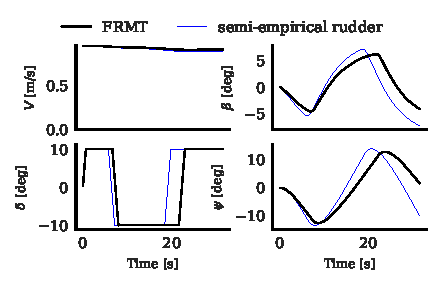
\includegraphics{figures/results_wPCC_ID.closed loop zigzag 10_10 port.pdf}
        \caption{Simulations wPCC Zigzag10/10 to port.}
        \label{fig:sim_wPCC_10}
     \end{subfigure}
     \vfill
     \begin{subfigure}[b]{\textwidth}
        \centering
        \includesvg{figures/results_wPCC_ID.closed loop zigzag 20_20 stbd.svg}
        \caption{Simulations wPCC Zigzag20/20 to starboard.}
        \label{fig:sim_wPCC_20}
     \end{subfigure}
        \caption{Comparison between zigzag tests with wPCC from experiments and simulations with a model equipped with semi-empirical rudder model.}
        \label{fig:sim_wPCC}
\end{figure}
%\begin{figure}[h]
%     \centering
%     \begin{subfigure}[b]{\textwidth}
%         \centering
%         \includesvg{figures/results_wPCC_ID.overshoot1.svg}
%        \caption{First overshoot angles.}
%        \label{fig:overhoots1_wPCC}
%     \end{subfigure}
%     \vfill
%     \begin{subfigure}[b]{\textwidth}
%         \centering
%         \includesvg{figures/results_wPCC_ID.overshoot2.svg}
%        \caption{Second overshoot angles.}
%        \label{fig:overhoots2_wPCC}
%     \end{subfigure}
%     
%        \caption{Overshoot angles from the wPCC experiments and simulations.}
%        \label{fig:overshoots_wPCC}
%\end{figure}